%!TEX root = practicum3.tex
To find the intersected edges and compute the intersection points we have used the method \t{find_intersected_edges}, see \autoref{lst:c:find_intersected_edges}. This method calls the method \t{line_segments_intersect} (\autoref{lst:b:intersectLineSegments}) on the edge defined by the points \t{p0} and \t{p1} and the edges of the triangulation. If an intersection is found it adds the indices of the intersected edge in the global list \t{intersected_line_segments} and appends the intersection point to \t{intersection_points}. The intersected edges of the triangulation and the intersection points are presented in \autoref{tab:c:intersectedEdges}.

\lstinputlisting[float, firstline=180, lastline=199, label={lst:c:find_intersected_edges}, caption={The method \t{find_intersected_edges()}.}]{../assignment3C.py}

To visualize the results we have added the code in \autoref{lst:c:display_1}, the resulting visualization is shown in \autoref{fig:c:result}.

\lstinputlisting[float, firstline=115, lastline=129, label={lst:c:display_1}, caption={Part of the method \t{display()} that visualizes the intersected edges and the intersections.}]{../assignment3C.py}

\begin{figure}
	\centering
	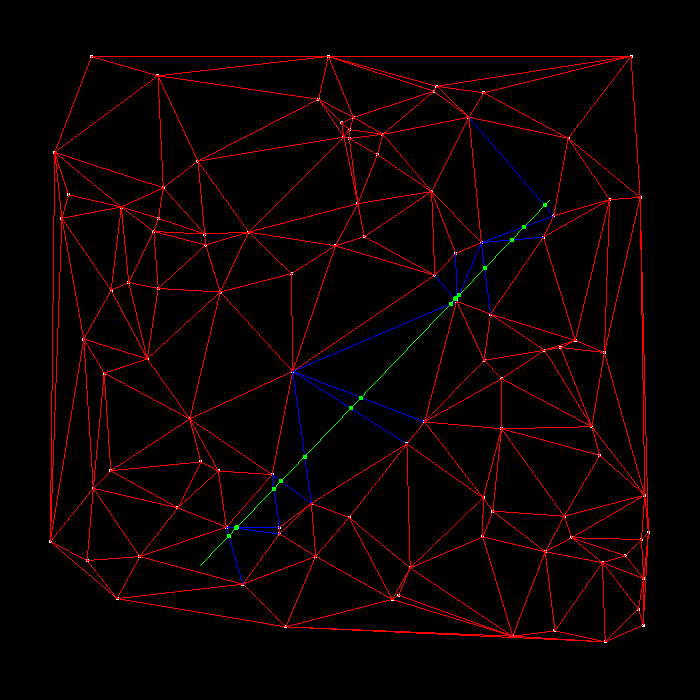
\includegraphics[width=0.5\textwidth]{./img/c_result}		
	\caption{The visualization of the intersection of the line segment $s$ with the edges of the triangulation $dt$. Each intersected edges is shown in blue, the green dots represent the intersections.}
	\label{fig:c:result}
\end{figure}


\begin{table}
	\centering
	\footnotesize{
		\begin{tabular}{ll|ll}
		edge & intersection & edge & intersection\\
		\hline
		(\num{226.33195013}, \num{527.007719279}) - (\num{242.796962849}, \num{584.179466813})	&	(\num{228.867696999}, \num{535.812636852})	&	 (\num{456.54758505}, \num{301.329564578}) - (\num{292.651351959}, \num{371.369188947})	&	(\num{450.717707067}, \num{303.820912038})	\\
		(\num{226.33195013}, \num{527.007719279}) - (\num{279.526723944}, \num{533.851551524})	&	(\num{236.087462036}, \num{528.262825414})	&	 (\num{434.746175446}, \num{275.228689898}) - (\num{456.54758505}, \num{301.329564578})	&	(\num{454.940291133}, \num{299.405295558})	\\ 
		(\num{226.33195013}, \num{527.007719279}) - (\num{279.230162351}, \num{527.629726937})	&	(\num{237.165877611}, \num{527.135110841})	&	 (\num{543.382588894}, \num{237.142130429}) - (\num{481.36728233}, \num{242.669629937})	&	(\num{511.78866886}, \num{239.958134849})	\\ 
		(\num{272.14012592}, \num{474.6185968}) - (\num{279.230162351}, \num{527.629726937})	&	(\num{274.010859273}, \num{488.60578716})	&	 (\num{481.36728233}, \num{242.669629937}) - (\num{490.590138248}, \num{314.176426186})	&	(\num{484.674568747}, \num{268.311736682})	\\ 
		(\num{272.14012592}, \num{474.6185968}) - (\num{311.312430627}, \num{503.369689707})	&	(\num{281.098731465}, \num{481.193897954})	&	 (\num{481.36728233}, \num{242.669629937}) - (\num{456.54758505}, \num{301.329564578})	&	(\num{459.283383215}, \num{294.863662123})	\\ 
		(\num{292.651351959}, \num{371.369188947}) - (\num{406.885957326}, \num{443.993258738})	&	(\num{350.781795159}, \num{408.325322776})	&	 (\num{455.757245676}, \num{253.484433518}) - (\num{456.54758505}, \num{301.329564578})	&	(\num{456.489045688}, \num{297.785740795})	\\ 
		(\num{292.651351959}, \num{371.369188947}) - (\num{311.312430627}, \num{503.369689707})	&	(\num{304.689843297}, \num{456.524335295})	&	 (\num{553.745608126}, \num{215.87226731}) - (\num{481.36728233}, \num{242.669629937})	&	(\num{524.448996513}, \num{226.719049361})	\\ 
		(\num{292.651351959}, \num{371.369188947}) - (\num{424.577450772}, \num{421.869738174})	&	(\num{361.075143445}, \num{397.561421426})	&	 (\num{468.981532514}, \num{117.202657047}) - (\num{553.745608126}, \num{215.87226731})	&	(\num{544.790307044}, \num{205.447850348})	\\	 	
		\end{tabular}
	}
	\caption{The edges that were intersected by the line segment between \t{p0} and \t{p1} and the point where the line segment intersected the edge. A point \vec{P} defined by its $x$ and $y$ coordinate is represented as $(x, y)$. A linesegment between the points \vec{P_1} and \vec{P_2} is represented as (\vec{P_1}, \vec{P_2}).}
	\label{tab:c:intersectedEdges}
\end{table}

~\\

\todo[inline]{Find and print the consecutive intersection points going from p0 to p1 without using the actual coordinates of the intersection points.}


